\chapter{Desenvolvimento}

Esta seção tem por propósito apresentar o estudo realizado sobre a
\textit{startup} Rua Dois Tecnologias, sendo esta o objeto de análise
central do presente trabalho. O escopo deste capítulo abrangerá desde
o entendimento sobre o contexto da empresa e sua proposta de valor
até aspectos mais técnicos como a arquitetura do sistema, sua evolução
durante o primeiro ano da empresa e as dificuldades enfrentadas pela
\textit{startup} nessa arquitetura.

  As seções estão dispostas em:

  \begin{enumerate}
    \item \textbf{Rua Dois Tecnologias:} breve apresentação sobre a empresa,
      seus propósitos e os serviços oferecidos;
    \item \textbf{Arquitetura do sistema:} descrição da arquitetura de software
      adotada dentro da Rua Dois, no seu primeiro ano de desenvolvimento, e possíveis
      soluções discutidas dentro da empresa a respeito da escalabilidade.
  \end{enumerate}

\section{Rua Dois Tecnologias}

No artigo \textit{Modernizing Real Estate: The Property Tech Opportunity}
\footnote{Disponível
\href{https://www.forbes.com/sites/valleyvoices/2019/02/22/the-proptech-opportunity}{nest link}.},
a autora \citeonline{LouisaXu} aborda uma visão histórica sobre o desenvolvimento
de tecnologias para o mercado imobiliário fazendo um comparativo com a realidade atual.
Nesse histórico de desenvolvimento, ela relata que desde 1980 são empregados
diversos esforços na área buscando melhorarias por meio de software, mas mesmo
assim, continuamos em uma ramo altamente burocrático e carente de melhorias.

Mediante essas limitações, surgiu em outubro de 2018 a Rua Dois Tecnologias,
com o propósito de solucionar as dificuldades enfrentadas tanto por parte das
imobiliárias quanto por parte dos locatários \footnote{Aquele que mora em um imóvel
que não lhe pertence, mediante um contrato de locação.} no processo de locação de imóveis.

A proposta\footnote{Mais informações a respeito da proposta e visão da Rua Dois podem
ser encontradas
\href{https://open.spotify.com/episode/2jYKPCPLCIdDWwxpR0theT?si=dT6WUG7JSEGJH3mVVIJitQ}
{neste \textit{podcast}}.}
da empresa consiste em atuar como um facilitador para as imobiliárias
ingressarem no meio digital e consequentemente propiciar seu crescimento. Para tal,
eles buscam aumentar a eficiência do processo de locação por meio da digitalização,
proporcionando melhor integração entre operação e tecnologias. Assim, com um processo
mais digital, os recursos humanos podem ser melhores empregados no atendimento do
cliente favorencendo a experiência do mesmo nesse mercado tão burocrático.


% Transformação Digital
%     Inovação é criar valor
%     Por meio de um processo mais digital entregar uma nova experiência para o usuário
%     com mais eficiência e podendo se adaptar a novos modelos de negócio
%     experiencia + eficiencia = novo modelo de negócio
%     nova intereção do time
%     digitalizacao markenting em vendas
%     digitalização de produto
%     liderança pela inovação
%     fisico-digital
%
%     burocracia enorme
%     perca de relacionamento com o cliente >> processo, automatizar, automatizar...
%     voltar a um relacionamento muito grande mas com um alto grau de tecnologia envolvido nesse
%     relacionamento entregando uma experiência melhor para o usuário e alcançando mais gente
%
%     dificuldade de crescer num mundo digital
%
%     proposito da rua dois: democratizar a experiência positiva de locação no brasil
%     integração muito grande entre operação e tecnologia >> processos
%     tecnologia + operação + serviço
%     validação >> estatisticas >> crescimento da empresa
%     lead >> direto para visita

% TODO Conversar com o Erlan para melhorar essa parte
% TODO Explicar o que é CEO e colocar nas lista de abreviações
% TODO Descrever melhor o contexto e os papeis envolvidos

\subsection{Serviços prestados}

Visando o processo de locação de imóveis, a Rua Dois conta com quatro serviços
sendo desenvolvidos dentro da empresa, afim de agregar valor aos seus clientes,
sendo eles:

  \begin{enumerate}
    \item \textbf{Captação de Imóveis:} serviço destinado à atrair proprietários de
      imóveis que desejam divulgar o imóvel para locação;
    \item \textbf{Visitas:} serviço de visitas aos imóveis, no qual os interessados em
      locar o imóvel agendam um horário para conhecer o mesmo;
    \item \textbf{Propostas:} serviço no qual os interessados, após passarem pela etapa
      de visitação, avaliam o imóvel e fazem uma proposta para o proprietário do
      imóvel referente ao valor a ser pago pela locação e possíveis ajustes que
      desejam que sejam feitos na propriedade;
    \item \textbf{Contrato:} etapa final, destinada a automatizar a avaliação por parte
      das seguradoras, envio de documentos e assinatura do contrato.
  \end{enumerate}

Cada serviço é vendido de forma separada para as imobiliárias, de forma que cada uma
adapte ao seu contexto os serviços que melhor se encaixam. Atualmente, o serviço
mais desenvolvido é o de visitas e a equipe vem trabalhando com o intuito de
estabilizar os demais serviços.

\section{Arquitetura do sistema}
\label{sec:ArquiteturaDoSistema}

O início do desenvolvimento do software da Rua Dois se deu em outubro de 2018 com
base na proposta de criar um sistema usando de uma arquitetura de microsserviços, de
forma que esse sistema já fosse preparado pra escalar desde seu início. Contudo,
a empresa enfrentou uma série de dificuldades\footnote{Estas dificuldades serão abordadas
com maior clareza na \autoref{sec:ArquiteturaFase1}} em relação a esta arquitetura e ao seu
contexto no respectivo momento. Mediante essas dificuldades a Rua Dois optou em seu
processo de desenvolvimento migrar essa arquitetura de microsserviços para um sistema
monolítico.

Esta seção visa descrever essas duas fases arquiteturais dentro da empresa com suas
respectivas motivações e desafios encontrados. Assim, visando facilitar o entendimento,
cada fase será nomeada da seguinte forma:

    \begin{description}
        \item [Fase 1] referente a fase inicial de desenvolvimento na qual foi adotada
        uma arquitetura de microsserviços;
        \item [Fase 2] referente a segunda fase de desenvolvimento na qual foi adotada
        uma arquitetura monolítica.
    \end{description}


\subsection{Arquitetura do sistema: Fase 1}
\label{sec:ArquiteturaFase1}

A primeira fase de desenvolvimento da \textit{startup} foi marcada pela premissa de
que o sistema deveria ser escalável, e com base nessa premissa foram tomadas uma
série de decisões visando preparar o sistema para tal. Assim o sistema foi dividido 
em dois microsserviços principais e em uma série de microsserviços auxiliares
distribuídos nos lambdas da \gls{AWS}. Os dois serviços principais são:

    \begin{description}
        \item [r2service] responsável por gerir o cadastro de imóveis e as propostas
        de locação do imóvel;
        \item [r2visit] responsável por gerir a lógica de agendamento de visitas
        a um imóvel.
    \end{description}

A \autoref{fig:ArquiteturaFase1} visa ilustrar a organização desse sistema. Nela
os dois serviços principais estão representados pelos círculos maiores roxos e as
demais representações são outros serviços que auxiliam no ciclo de vida do produto.
Adiante segue descrito o fluxo com o qual todo o sistema é acionado, seguindo a
enumeração disposta na imagem:

\begin{figure}[h]
  \centering
  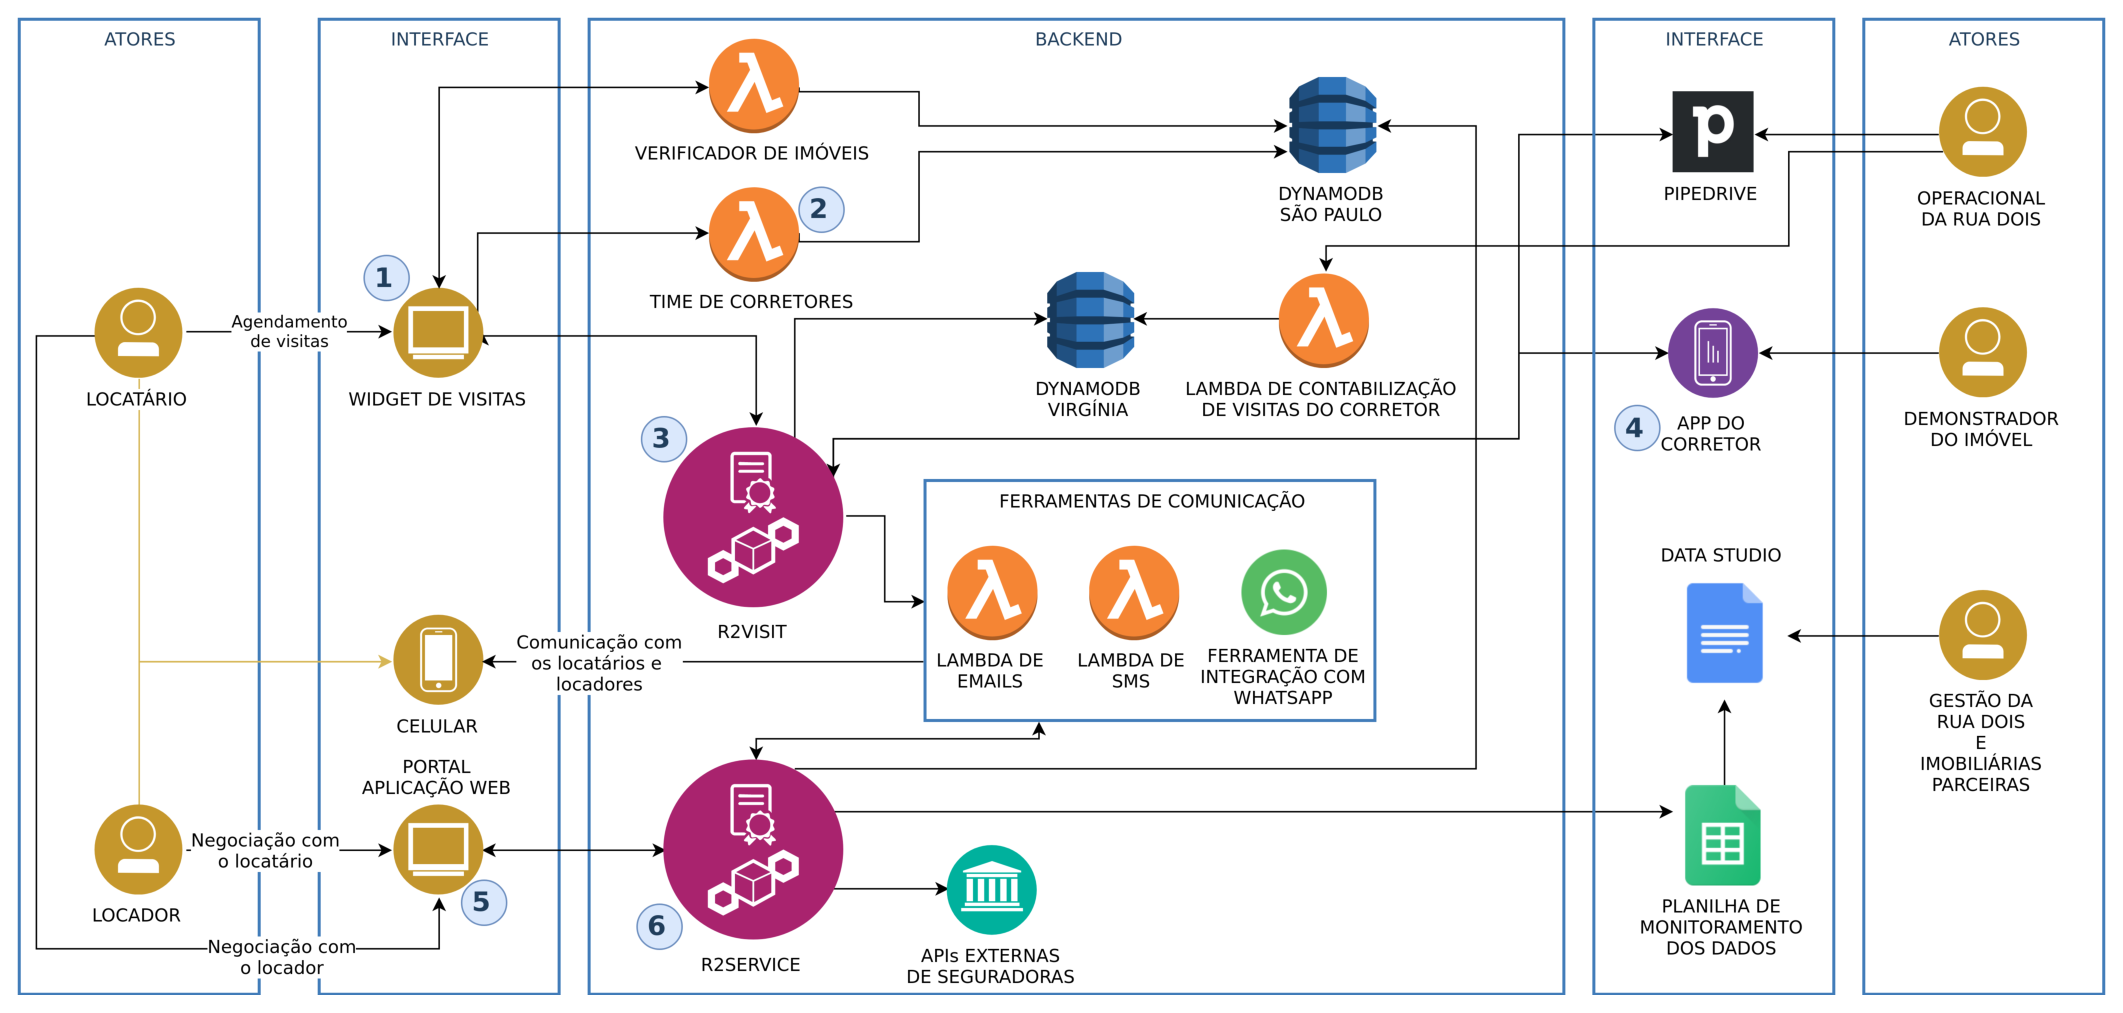
\includegraphics[keepaspectratio=true,scale=0.4]{figuras/r2ArquiteturaFase1.eps}
  \caption{Arquitetura do sistema da Rua Dois na Fase 1\label{fig:ArquiteturaFase1}}
\end{figure}

  \begin{enumerate}
    \item O \textit{Widget} é um componente utilizado pela Rua Dois que roda
      no \textit{frontend} dos sites das imobiliárias que aderem ao serviço
      de visitas. Ele se comunica com um lambda responsável por verificar se
      o imóvel apresentado no site da imobiliária está disponível no banco
      de dados da Rua Dois. Uma vez que esteja disponível, o \textit{widget}
      exibe um botão que disponibiliza o agendamento da visita \textit{online}
      para o interessado;
    \item O locatário ao clicar nesse botão, dispara uma requisição ao lambda
    que identifica o time de corretores responsável por atender as visitas
    ao imóvel selecionado. E em seguida, uma nova requisição é disparada ao
    serviço \textit{r2visit} solicitando o calendário com os horários
    disponíveis do respectivo time;
    \item Após o locatário ter selecionado o horário da visita, uma nova
    requisição é lançada para registrar a visita no \textit{r2visit}, que por
    sua vez dispara uma série de mensagens por meio das ferramentas de comunicação
    e atualiza o Pipedrive\footnote{O Pipedrive é uma ferramenta de \gls{CRM} utilizada pela
    empresa para realizar o gerenciamento operacional e monitoramento dos resultados obtidos.
    Saiba mais em: \url{https://www.pipedrive.com}};
    \item Após a visita ser realizada, o corretor sinaliza por meio do aplicativo
    a conclusão da visita, disparando novamente no \textit{r2visit} os eventos
    de atualização do Pipedrive e as ferramentas de comunicação, para que se
    possa dar início a nova fase de Negociação, referente ao produto de propostas;
    \item Nessa nova fase, locatário e locador trocam mensagens por meio do portal
    da Rua Dois, o qual é gerido pelo \textit{r2service}. Ao final da negociação,
    os clientes entram na fase de contrato, na qual seu dados são recolhidos e
    enviados por meio do \textit{r2service} para \glspl{API} externas de seguradoras as quais
    realizam uma avaliação de crédito do locatário. Quando concedida a avaliação
    de crédito, o contrato é gerado automaticamente com os dados já recolhidos
    do locatário, locador, da imobiliária e do próprio imóvel;
    \item Por fim, o \textit{r2service} é responsável por atualizar uma planilha do
    Google Sheets\footnote{Saiba mais em: \url{https://www.google.com/sheets/about/}}
    que serve de insumo para geração de relatórios dentro do Data Studio
    \footnote{Saiba mais em: \url{https://datastudio.google.com}}.
  \end{enumerate}

Nesse fluxo nota-se que existe uma grande diversidade de elementos interagindo entre
si e a forma como isto foi organizado gerou as seguintes dificuldades dentro da empresa:

    \begin{enumerate}
        \item{Dificuldade de organização dos dados da empresa uma vez que não houve
        um bom planejamento em relação a interação entre os serviços \textit{r2service}
        e \textit{r2visit}, o que ocasionou a duplicação da tabela referente aos dados
        dos imóveis - uma tabela no banco de dados da Virgínia e a outra tabela no banco
        de dados de São Paulo;}
        \item{Dificuldade de gerir as associações necessárias entre os dados armazenados
        no banco. A empresa optou pelo uso do banco não relacional DynamoDB, visando
        novamente a escalabilidade, mas sem planejar corretamente o armazenamento desses
        dados nessa estrutura não relacional. Isso impactou diretamente o desenvolvimento,
        visto que existe uma necessidade da empresa de tratar esse dado como relacional
        mas fez isso em cima de uma tecnologia inadequada para tal;}
        \item{Dificuldade de manter essa infraestrutura, tanto pela complexidade na forma
        como o sistema está organizado quanto pela escolha de utilizar a infraestrutura da
        \gls{AWS}, que é mais árdua de trabalhar do que outras soluções disponíveis no mercado
        \cite{kavya};}
        \item{Dificuldade de inserção de novos membros na equipe de desenvolvimento, visto
        que entender como esses vários serviços se relacionam não é uma tarefa simples;}
        \item{Dificuldade de mudança e inserção de novas funcionalidades. Nessa primeira
        fase a Rua Dois encontrava-se fortemente no período de validação da ideia dentro
        de uma \textit{startup} o que exigia uma rápida reação da equipe em relação aos
        \textit{feedbacks} recebidos. Contudo, nessa arquitetura se tornou exaustivo a
        realização de constantes mudanças vistos todos os problemas relatados nos tópicos
        anteriores.}
    \end{enumerate}

% Desde seu início, a Rua Dois tem em seu modelo de negócio uma constante
% preocupação com a escalabilidade do sistema. A empresa tem em seus objetivos
% validar rapidamente a ideia e expandir para diferentes mercados. Contudo,
% este objetivo foi alinhado a uma equipe de desenvolvimento de software
% inexperiente tanto no contexto de desenvolver software para \textit{startups}
% quanto em questões de qualidade e arquitetura de software. A soma desses
% dois fatores gerou uma série de decisões equivocadas sobre a arquitetura
% desse sistema que hoje atrapalham sua evolução ao invés de facilitar o
% crescimento escalável da empresa. Dentre estas decisões estão:
%
%   \begin{enumerate}
%     \item A escolha de usar um banco não-relacional - DynamoDB - em um
%     contexto extremamente relacional. Atualmente existem seis entidades
%     principais dentro do sistema: imobiliária, imóvel, cliente, corretor,
%     visita e proposta. Todas dispostas em tabelas diferentes do DynamoDB,
%     o que implica que todos os relacionamentos entre as entidades são
%     construídos a nível de aplicação. A documentação do DynamoDB diz:
%       \begin{quotation}
%         "Em geral, você deve manter o mínimo de tabelas possível em um
%         aplicativo do DynamoDB. A maioria dos aplicativos bem-projetados exige
%         somente uma tabela." \cite{doc:dynamodbModeling}.
%       \end{quotation}
%     A Rua Dois foi contrária a essa recomendação, e trabalha com uma tabela
%     para cada entidade. De forma que, toda a eficiência que eles
%     buscavam em fazer consultas com um banco de dados \gls{NoSQL}, é perdida
%     no mal planejamento do projeto em cima desse arquitetura.
%     \item A adoção de microsserviços sem conhecer a real demanda dos
%     serviços que seriam oferecidos. Sendo uma \textit{startup}, a Rua Dois
%     se caracteriza por um ambiente extremante incerto, de validação de ideias.
%     Oleksiy Kovyrin, chefe do Swiftype\footnote{\url{https://swiftype.com/}},
%     disse em entrevista a \citeonline{JakeLumetta}:
%       \begin{quotation}
%         "Toda vez que consideramos a introdução de um novo serviço, temos que
%         considerar o custo operacional de fazer isso. Cada novo serviço aumenta a
%         complexidade da infraestrutura e torna um pouco mais difícil raciocinar
%         sobre as relações de serviço dentro do sistema."
%       \end{quotation}
%     Dado o contexto da Rua Dois, no qual não se tem domínio sobre o produto final
%     que será entregue somado a uma equipe sem experiência de trabalho com microsserviços,
%     a escolha mais segura seria um sistema monolítico \cite{JakeLumetta}.
%     Atualmente, a empresa enfrenta dificuldades de manter essa arquitetura,
%     compartilhar o conhecimento sobre a mesma com novos integrantes e, principalmente,
%     manter a consistência dos dados. Esse último é o fator de maior impacto
%     na arquitetura, uma vez que se tem diversos microsserviços compartilhando
%     o uso das mesmas tabelas, além de tabelas duplicadas em serviços diferentes,
%     nas quais é necessário estar realizando constantemente a sincronização dos dados.
%
%     \item Optar por usar a infraestrutura na Amazon Web Services, a qual
%     possui diversos recursos mas também possui maior complexidade para
%     configurá-los do que outras ferramentas disponíveis no mercado \cite{kavya}.
%     Completando o quadro de utilizar uma arquitetura de microsserviços, com
%     uma equipe inexperiente, a empresa ainda enfrenta as dificuldades de manter
%     essa arquitetura que não é trivial, em uma infraestrutura que também exige
%     determinados conhecimentos que atualmente o time de desenvolvimento
%     não possui.
%   \end{enumerate}

% Não é preciso o widget solicitar o time, o r2visit deve ser capaz de fazer isso pelo imóvel

\subsection{Arquitetura do sistema: Fase 2}

Mediante as dificuldades enfrentadas na arquitetura adotada na Fase 1 e a
incerteza sobre a escalabilidade desse sistema, em junho de 2019 a Rua Dois
optou por migrar para uma arquitetura monolítica com a perspectiva de tornar
o sistema mais estável e mais apto a realização de mudanças. Nessa mudança
os serviços \textit{r2service} e \textit{r2visit} se tornaram um único sistema,
agora chamado de \textit{novo r2service}, alguns lambdas foram incorporados por
esse novo sistema ou simplesmente foram descartados juntamente com alguns
serviços auxiliares que não seriam mais usados. A \autoref{fig:ArquiteturaFase2}
exemplifica como está o sistema nessa nova configuração.

\begin{figure}[h]
  \centering
  \includegraphics[keepaspectratio=true,scale=0.3]{figuras/r2ArquiteturaFase2.eps}
  \caption{Arquitetura do sistema da Rua Dois na Fase 2\label{fig:ArquiteturaFase2}}
\end{figure}
